% A mindmap showing TeX online projects supported
% by DANTE e.V. which sponsors their server costs.
% Author: Stefan Kottwitz
\documentclass[border=10pt]{standalone}
\usepackage[utf8]{inputenc}
\usepackage{dtklogos}
\usepackage{tikz}
\usetikzlibrary{mindmap,shadows}
\usepackage[hidelinks,pdfencoding=auto]{hyperref}
% Information boxes
\newcommand*{\info}[4][16.3]{%
  \node [ annotation, #3, scale=0.65, text width = #1em,
          inner sep = 2mm ] at (#2) {%
  \list{$\bullet$}{\topsep=0pt\itemsep=0pt\parsep=0pt
    \parskip=0pt\labelwidth=8pt\leftmargin=8pt
    \itemindent=0pt\labelsep=2pt}%
    #4
  \endlist
  };
}
\begin{document}
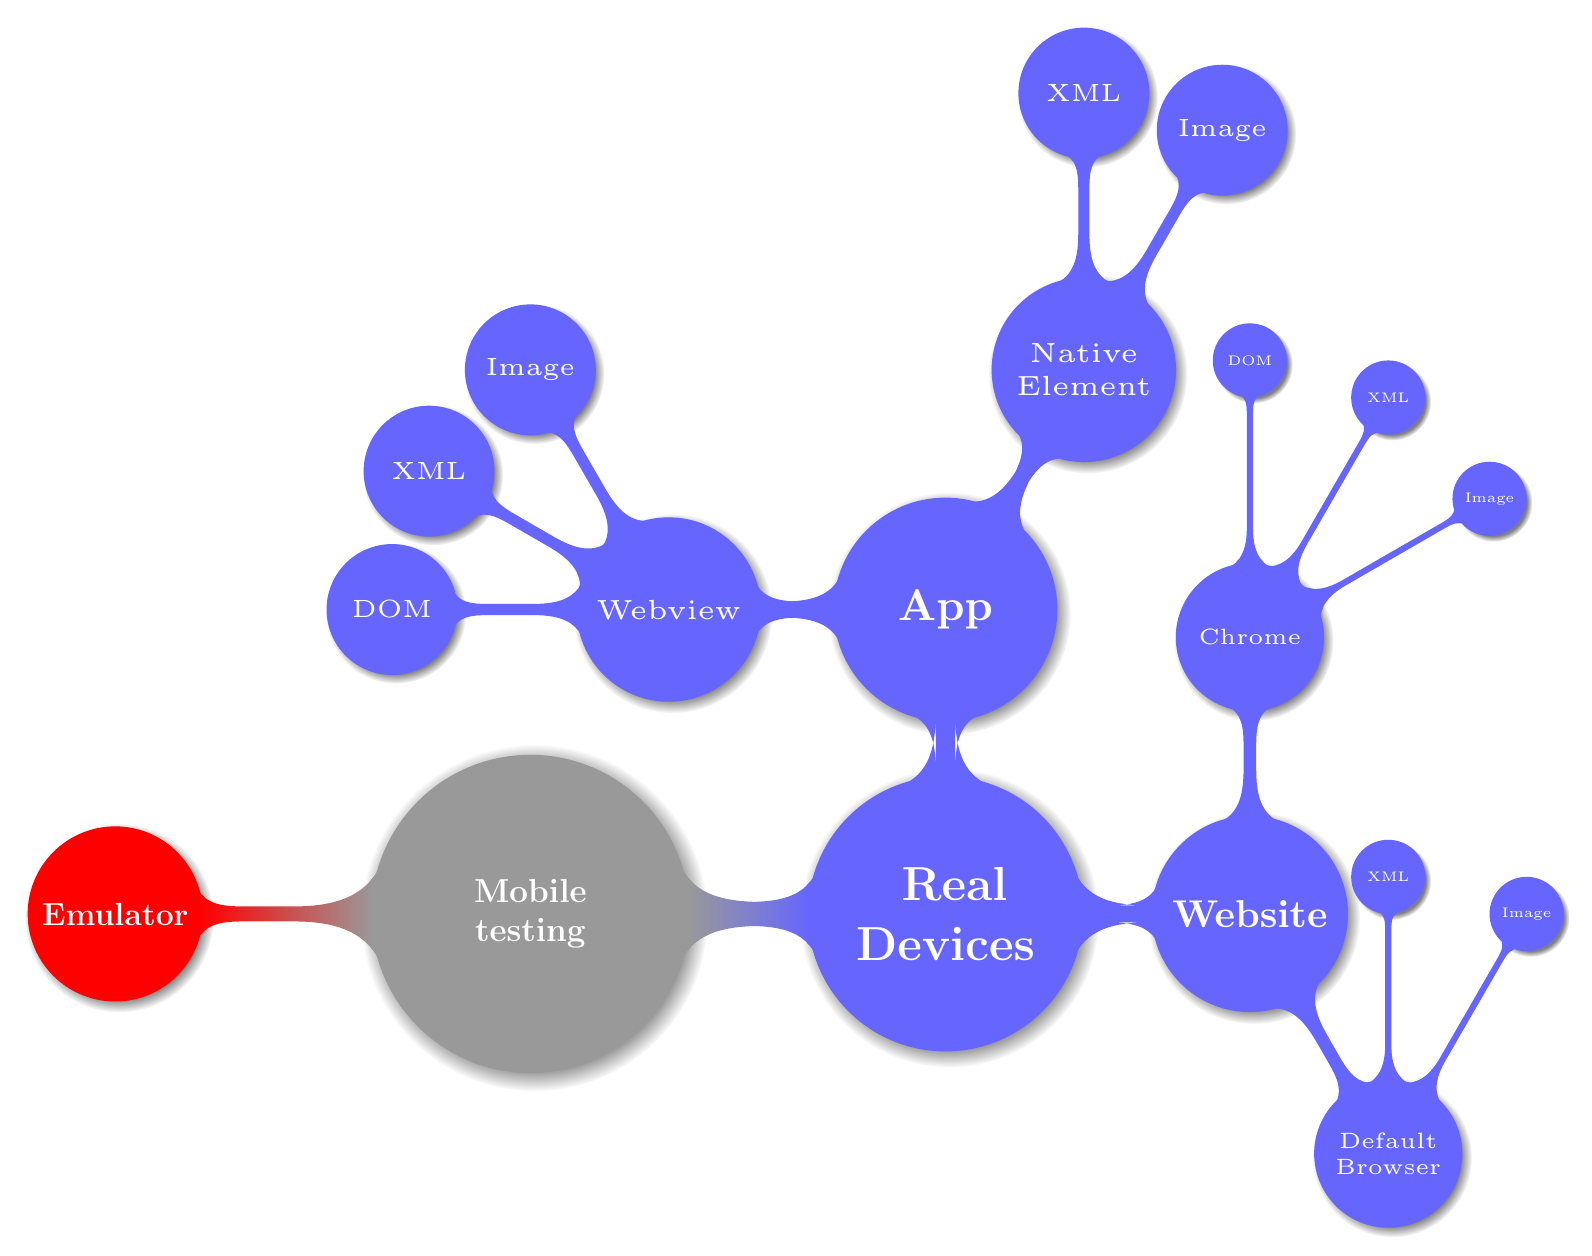
\begin{tikzpicture}[ every annotation/.style = {draw,
                     fill = white, font = \Large}]
  \path[mindmap,concept color=black!40,text=white,
    every node/.style={concept,circular drop shadow},
    root/.style    = {concept color=black!40,
      font=\large\bfseries,text width=10em},
    level 1 concept/.append style={font=\Large\bfseries,
      sibling angle=180, text width=7.7em, level distance=15em,inner sep=0pt},
    level 2 concept/.append style={font=\bfseries,level distance=11em, sibling angle=90},
    level 3 concept/.append style={level distance=10em},
    level 4 concept/.append style={level distance=10em},
  ]
  node[root] {Mobile\\testing} [clockwise from=0]
    child[concept color=blue!60] {
      node[concept, scale=1.2] {{ Real Devices }} [clockwise from=90]
        child { node[concept, scale=1.6] (App) {App}
                child[sibling angle=120, rotate=90] { node[concept, scale=2.0] (appwebview) {Webview} 
                        child { node[concept, scale=1.8] {DOM} }
                        child { node[concept, scale=1.8] {XML} }
                        child { node[concept, scale=1.8] {Image} }
                      }
                child { node[concept, scale=2.0] {Native\\Element}
                        child { node[concept, scale=1.8] {XML} }
                        child { node[concept, scale=1.8] {Image} }
                      }
              }
        child { node[concept, scale=1.4] (Website) {Website}
                child[sibling angle=30] { node[concept, scale=1.6] (sitewebchrome) {Chrome}
                        child { node[concept] {DOM} }
                        child { node[concept] {XML} }
                        child { node[concept] {Image} }
                      }
                child[sibling angle=150] { node[concept, scale=1.6] (sitewebdefault) {Default\\Browser}
                        child { node[concept] {XML} }
                        child { node[concept] {Image} }
                      }
              }
    }
    child[concept color=red] {
      node[concept, scale=0.8] (Emulator) {{Emulator}}
      [clockwise from=270]
    };
\end{tikzpicture}
\end{document}